\subsubsection{Deep Feedforward Networks}

\begin{remark} \hlt{Deep Feedforward Networks (DFNs)}\\
Defines a mapping $\bm{y} = f(\bm{x}; \bm{\theta})$ and learns value of parameters $\bm{\theta}$ that results in best function approximation.
\end{remark}

\begin{remark} \hlt{Linear Models}\\
Linear models may fit data efficiently and reliably, either in closed form or with convex optimisation.\\
Model capacity limited to linear functions, does not model interaction between any two input variables
\end{remark}

\begin{remark} \hlt{Nonlinear Models}\\
To represent nonlinear functions of $\bm{x}$, apply linear model to transformed input $\phi(\bm{x})$ where $\phi$ is a nonlinear transformation. Kernel trick may be applied to obtain nonlinear learning algorithm. To choose mapping $\phi$:
\begin{enumerate}[label=\roman*.]
\setlength{\itemsep}{0pt}
\item Choose generic $\phi$, such as that used by kernel machines based on RBF kernel.\\
If $\phi(\bm{x})$ is of high enough dimension, can find enough capacity to fit training set, but generalisations to test set remains poor. Mappings are based on principle of local smoothness and do not encode enough prior information to solve advanced problems.
\item Manually engineer $\phi$. Requires decades of human effort for each task, and practitioners specialising in different domains (i.e, speech recognition, computer vision) with little transfer between domains.
\item Learn $\phi$ through deep learning. Model is $y = f(\bm{x}; \bm{\theta}, \bm{w}) = \phi(\bm{x}; \bm{\theta})^T \bm{w}$, where parameters $\bm{\theta}$ can be used to learn $\phi$ from broad class of functions, and parameters $\bm{w}$ that map from $\phi(\bm{x})$ to desired output.\\
Do not require training problem to be convex, and only require finding the right general function.
\end{enumerate}
\end{remark}

\begin{definition} \hlt{Cost Functions}
\begin{enumerate}[label=\roman*.]
\setlength{\itemsep}{0pt}
\item Learning Conditional Distributions with Maximum Likelihood: cost function is negative log-likelihood, which is the cross-entropy between training data and model distribution:
\begin{equation}
J(\bm{\theta}) = - \mathbb{E}_{\bm{x}, \bm{y} \sim \hat{p}_{\text{data}}} \log p_{\text{model}}(\bm{y} \ \vert \ \bm{x}) \nonumber
\end{equation}
Specific form of cost function changes from model to model, depending on form of $\log p_{\text{model}}$.\\
Method removes the burden of designing cost functions for each model, as specifying a model $p(\bm{y} \ \vert \ \bm{x})$ automatically determines a cost function $\log p(\bm{y} \ \vert \ \bm{x})$.
\item Learning Conditional Statistics: to learn just one conditional statistic of $\bm{y}$ given $\bm{x}$.\\
With sufficiently powerful neural network, this can represent any function $f$ from a wide class of function, limited by features of continuity and boundedness. Hence the cost function is a functional. Learning is choosing a functional rather than a set of parameters.\\
By calculus of variable, solving the optimisation problem yields the below function,
\begin{align}
f^* &= \arg \min_f \mathbb{E}_{\bm{x}, \bm{y} \sim p_{\text{data}}} \Vert \bm{y} - f(\bm{x}) \Vert^2 \nonumber \\
f^* &= \mathbb{E}_{\bm{y} \sim p_{\text{data}}(\bm{y} \ \vert \ \bm{x})} [\bm{y}] \nonumber
\end{align}
If infinitely many samples from the true data-generating distribution could be trained, then minimising the mean squared error cost function gives a function that predicts mean of $\bm{y}$ for each value of $\bm{x}$.\\
A second result from calculus of variations is:
\begin{align}
f^* = \arg \min_f \mathbb{E}_{\bm{x}, \bm{y} \sim p_{\text{data}}} \Vert \bm{y} - f(\bm{x}) \Vert_1 \nonumber
\end{align}
which is a function that predicts the median value of $\bm{y}$ for each $\bm{x}$. This is the mean absolute error.\\
Note that mean squared error and mean absolute error often lead to poor results when used with gradient-based optimisation. Output units that saturate may produce very small gradients when combined with these cost functions. Hence the reason that cross-entropy cost function is more popular.
\end{enumerate}
\end{definition}

\begin{definition} \hlt{Output Units}
\begin{enumerate}[label=\roman*.]
\setlength{\itemsep}{0pt}
\item Linear Units: base on affine transformation with no nonlinearity.\\
Given features $\bm{h}$, a layer of output units produces vector $\hat{\bm{y}} = \bm{W}^T \bm{h} + \bm{b}$. Linear output layers are used to produce mean of conditional Gaussian distribution:
\begin{equation}
p(\bm{y} \ \vert \ \bm{x}) = \mathcal{N}(\bm{y}; \hat{\bm{y}}, \bm{I}) \nonumber
\end{equation}
Maximising log-likelihood is equivalent to minimising mean squared error.\\
Linear units do not saturate, hence may be used for wide variety of optimisation algorithms.
\item Sigmoid Units: define Bernoulli distribution $y$ conditioned on $\bm{x}$. Neural net to predict $P(y = 1 \ \vert \ \bm{x})$, which lies in interval $[0,1]$. The sigmoid unit is defined by
\begin{equation}
\hat{y} = \sigma(\bm{w}^T \bm{h} + b) \nonumber
\end{equation}
where $\sigma$ is the logistic sigmoid function.\\
Note that the cost function used with maximum likelihood is $- \log P(y \ \vert \ \bm{x})$, preventing saturation.\\
The loss function for MLE of Bernoulli parametrised by sigmoid is
\begin{equation}
J(\bm{\theta}) = - \log P(y \ \vert \ \bm{x}) = - \log \sigma((2y - 1)z) = \zeta((1-2y)z) \nonumber
\end{equation}
Function saturates only when $(1-2y)z$ is very negative, i.e., when model has the right answer.
\item Softmax Units: used to represent probability distribution over $n$ different classes.\\
A linear layer predicts unnormalised log probabilities:
\begin{equation}
\bm{z} = \bm{W}^T \bm{h} + \bm{b} \nonumber
\end{equation}
where $z_i = \log \tilde{P}(y=i \ \vert \ \bm{x})$. Softmax function is then
\begin{equation}
\text{softmax}(\bm{z})_i = \frac{\exp(z_i)}{\sum_j \exp(z_j)} \nonumber
\end{equation}
The function is to maximise $\log P(y=i ; \bm{z}) = \log \text{softmax}(\bm{z})_i = z_i - \log \sum_{j} \exp(z_j)$.\\
Note that the input $z_i$ always has direct contribution to cost function, and the term cannot saturate.\\
Un-regularised maximum likelihood will drive the model to learn parameters that drive the softmax to predict fraction of counts for each outcome observed in the training set:
\begin{equation}
\text{softmax}(z(\bm{x}; \bm{\theta}))_i \approx \frac{\sum\limits_{j=1}^{m} \bm{1}_{y^{(j)}=i, \bm{x}^{(j)} = x}}{\sum\limits_{j=1}^m \bm{1}_{\bm{x}^{(j)}=x}} \nonumber
\end{equation}
Note that objective functions other than log-likelihood does not work well with softmax function. Squared error is poor loss function for softmax units, and can fail to train the model to change its output.\\
Softmax function can saturate, and many functions based on softmax also saturate, unless they are able to invert the saturating activating function.
\item Other Output Types: generally, given a conditional distribution $p(\bm{y} \ \vert \ \bm{x}; \ \bm{\theta})$, principle of maximum likelihood suggests using $- \log p(\bm{y} \ \vert \ \bm{x}; \ \bm{\theta})$ as the cost function.\\
Neural networks represent a function $f(\bm{x}; \bm{\theta}) = \bm{\omega}$. The outputs of the function are not direct predictions of value $\bm{y}$, but the parameters for distribution over $\bm{y}$. The loss function is then $- \log p(\bm{y} ; \bm{\omega}(\bm{x}))$.
\end{enumerate}
\end{definition}

\begin{remark} \hlt{Learning Distribution Parameters}
\begin{enumerate}[label=\roman*.]
\setlength{\itemsep}{0pt}
\item Heteroscedastic Model: to predict different variance in $\bm{y}$ for different values of $\bm{x}$, formulate the Gaussian distribution using precision rather than variance. In multi-variate case, the diagonal precision matrix is used, $\text{diag}(\bm{\beta})$. The log-likelihood of Gaussian distribution parametrised by $\bm{\beta}$ involves only multiplication by $\beta_i$ and addition of $\log \bm{\beta}_i$. The gradient of these operations are well-behaved.\\
Let $\bm{\alpha}$ be raw activation of the model used to determine diagonal precision. The softplus function may be used to obtain a positive precision vector $\bm{\beta} = \zeta(\bm{\alpha})$. Same strategy applies equally if using variance variance or standard deviation rather than precision.\\
If covariance is full and conditional, then parametrisation must be chosen that guarantees positive-definiteness of predicted covariance matrix.
\begin{equation}
\bm{\Sigma}(\bm{x}) = \bm{B}(\bm{x}) \bm{B}^T(\bm{x}) \nonumber
\end{equation}
where $\bm{B}$ is unconstrained square matrix. Note that if matrix is full rank, then computing likelihood requires $O(d^3)$ a $d \times d$ matrix for the determinant and inverse of $\bm{\Sigma}(\bm{x})$.
\item Mixture Density Networks: to perform multimodal regression (predict real values that come from conditional distribution $p(\bm{y} \ \vert \ \bm{x})$ that can have several different peaks in $\bm{y}$ for the same $\bm{x}$.
\begin{equation}
p(\bm{y} \ \vert \ \bm{x}) = \sum\limits_{i=1}^n p(c=i \ \vert \ \bm{x}) \mathcal{N}(\bm{y}; \bm{\mu}^{(i)} (\bm{x}), \bm{\Sigma}^{(i)} (\bm{x})) \nonumber
\end{equation}
The neural network will have three outputs:
\begin{enumerate}[label=\arabic*.]
\setlength{\itemsep}{0pt}
\item Mixture components $p(c = i \ \vert \ \bm{x})$, forming a multinoulli distribution over $n$ different components with latent variable $c$, obtained by softmax over $n$-dimensional vector.
\item Means $\bm{\mu}^{(i)}(\bm{x})$
\item Covariances $\bm{\Sigma}^{(i)}(\bm{x})$
\end{enumerate}
Gradient-based optimisation of conditional Gaussian mixtures can be unreliable as the divisions can be numerically unstable. May be solved by clipping gradients, or scaling gradients heuristically.
\end{enumerate}
\end{remark}

\begin{definition} \hlt{Hidden Units}\\
Even if hidden units are not differentiable at all input points, gradient descent still performs well enough as the training algorithms do not usually arrive at local minimum of cost function, but reduce its value significantly.\\
Most hidden units has input vector $\bm{x}$, computes an affine transformation $\bm{z} = \bm{W}^T \bm{x} + \bm{b}$, then applying element-wise non-linear function $g(\bm{z})$.
\begin{enumerate}[label=\roman*.]
\setlength{\itemsep}{0pt}
\item Rectified Linear Units (ReLUs): uses activation function $g(z) = \max \{0, z\}$.\\
Typically used on top of an affine transformation $\bm{h} = g(\bm{W}^T \bm{x} + \bm{b})$. In initialisation, set all elements of $\bm{b}$ to small positive values, so that ReLUs will be initially active for most inputs in training set.\\
Generalisations of ReLUs have non-zero slope $\alpha_i$ for $z_i < 0$: $h_i = \max(0, z_i) + \alpha_i \min(0, z_i)$.
\begin{enumerate}[label=\arabic*.]
\setlength{\itemsep}{0pt}
\item Absolute Value Rectification: sets $\alpha_i = -1$ to obtain $g(z) = \abs{z}$. Used for object recognition from images, to seek features that are invariant under polarity reversal of input illumination.
\item Leaky ReLU: fixes $\alpha_i$ to small positive value
\item Parametric ReU: treats $\alpha_i$ as a learnable parameter
\end{enumerate}
\item Maxout Units: divide $\bm{z}$ into groups of $k$ values. Each maxout unit then outputs maximum element of one of these groups: $g(\bm{z})_i = \max_{j \in \mathbb{G}^{(i)}} z_j$, where $\mathbb{G}^{(i)}$ is indices of inputs for group $i$, which is $\{(i-1)k + 1, \ldots, ik\}$.\\
This allows learning of piecewise linear function that responds to multiple directions in input $\bm{x}$ space .\\
Maxout units learn the activation function itself. With large $k$, maxout unit can learn to approximate any convex function. Each maxout unit is parametrised by $k$ weight vectors, hence need more regularisation than ReLUs. Benefits include:
\begin{enumerate}[label=\arabic*.]
\setlength{\itemsep}{0pt}
\item Can work well without regularisation if training set is large and number of pieces per unit is low.
\item Can gain statistical and computation advantages by requiring fewer parameters.
\item Have redundancy that resists catastrophic forgetting, where neural networks forgot how to perform tasks that were trained on in the past.
\end{enumerate}
\item Logistic Sigmoid and Hyperbolic Tangent: the logistic sigmoid activation function is $g(z) = \sigma(z)$, and the hyperbolic tangent activation function is $g(z) = \tanh(z)$. Note that $\tanh(z) = 2 \sigma(2z) - 1$.\\
Sigmoidal units saturate across most of the domain, which makes gradient-based learning very difficult. Hence the use in hidden units in feedforward networks is now discouraged.\\
If sigmoidal activation function must be used, hyperbolic tangent activation function performs better, as it resembles identity function more closely. Training $\hat{y} = \bm{w}^T \tanh(\bm{U}^T \tanh(\bm{V}^T \bm{x}))$ resembles training a linear model $\hat{y} = \bm{w}^T \bm{U}^T \bm{V}^T \bm{x}$ as long as the activations of the network can be kept small.\\
Sigmoidal functions are more common in recurrent networks, probabilities models, auto-encoders
\item Linear Unit: consider neural network layer with $n$ inputs, $p$ outputs, $\bm{h} = g(\bm{W}^T \bm{x} + \bm{b})$. Replace with two layers, one using weight matrix $\bm{U}$ and the other using weight matrix $\bm{V}$. If first layer has no activation function, then the factored approach is to compute $\bm{h} = g(\bm{V}^T \bm{U}^T \bm{x} + \bm{b})$. If $\bm{U}$ produces $q$ outputs, then $\bm{U}$ and $\bm{V}$ together only contains $(n+p)q$ parameters, while $\bm{W}$ contains $np$ parameters. For small $q$, this is considerable saving in parameters, while the cost is constraining linear transformation to be low rank. This is an efficient way of reducing number of parameters in the model.
\item Softmax: naturally represent probability distribution over discrete variable with $k$ possible values. Used only in more advanced architectures that explicitly learn to manipulate memory.
\item Radial Basis Function (RBF): function becomes more active as $\bm{x}$ approaches a template $\bm{W}_{:, i}$. As it saturates to $0$ for most $\bm{x}$, it can be difficult to optimise.
\begin{equation}
h_t = \exp \left( - \frac{1}{\sigma^2_i} \Vert \bm{W}_{:, i} - \bm{x} \Vert^2 \right) \nonumber
\end{equation}
\item Softplus: smooth version of rectifier for functional approximation and for conditional distributions of undirected probabilistic models. Usage is generally discouraged.
\begin{equation}
g(a) = \zeta(a) = \log(1 + e^a) \nonumber
\end{equation}
\item Hard $\tanh$: shaped similarly to $\tanh$ but bounded.
\begin{equation}
g(a) = \max(-1, \min(1,a)) \nonumber
\end{equation}
\end{enumerate}
\end{definition}

\begin{theorem} \hlt{Universal Approximation Theorem}\\
A feedforward network with linear output layer and at least one hidden layer with any 'squashing' activation function can approximate any Borel measurable function from one finite-dimensional space to another with any desired non-zero amount of error, provided the network is given enough hidden units.
\end{theorem}

\begin{method} \hlt{Architecture Design}\\
Neural network layers are arranged in a chain structure, with each layer being a function of preceding layer.
\begin{align}
\bm{h}^{(1)} &= g^{(1)} (\bm{W}^{(1)T} \bm{x} + \bm{b}^{(1)}) \nonumber \\
\bm{h}^{(k)} &= g^{(k)} (\bm{W}^{(k)T} \bm{h}^{(k-1)} + \bm{b}^{(k)}), \ \ \ k \geq 2 \nonumber
\end{align}
The main considerations are the depth of network and width of each layer. Deeper networks use far fewer units per layers and far fewer parameters, and often generalise to the test set, but are harder to optimise.
\end{method}

\begin{remark} \hlt{Depth of Network and Universal Approximation Theorem}\\
A feedforward network with single layer is sufficient to represent any function, but the layer may be infeasibly large and fail to learn and generalise correctly. Using deeper models can reduce number of units required to represent the desired function and can reduce generalisation error.\\
Shallow networks with broad family of non-polynomial activation functions have universal approximation properties. Piecewise linear networks can represent functions with number of regions that is exponential to depth.\\
The number of linear regions carved out by deep rectifier network with $d$ inputs, depth $l$, and $n$ units per hidden layer is $O(\binom{n}{d}^{d(d-1)} n^d)$. For maxout networks with $k$ filters per unit, this is $O(k^{(k-1)+d})$.
\end{remark}

\begin{figure}[H]
\centering
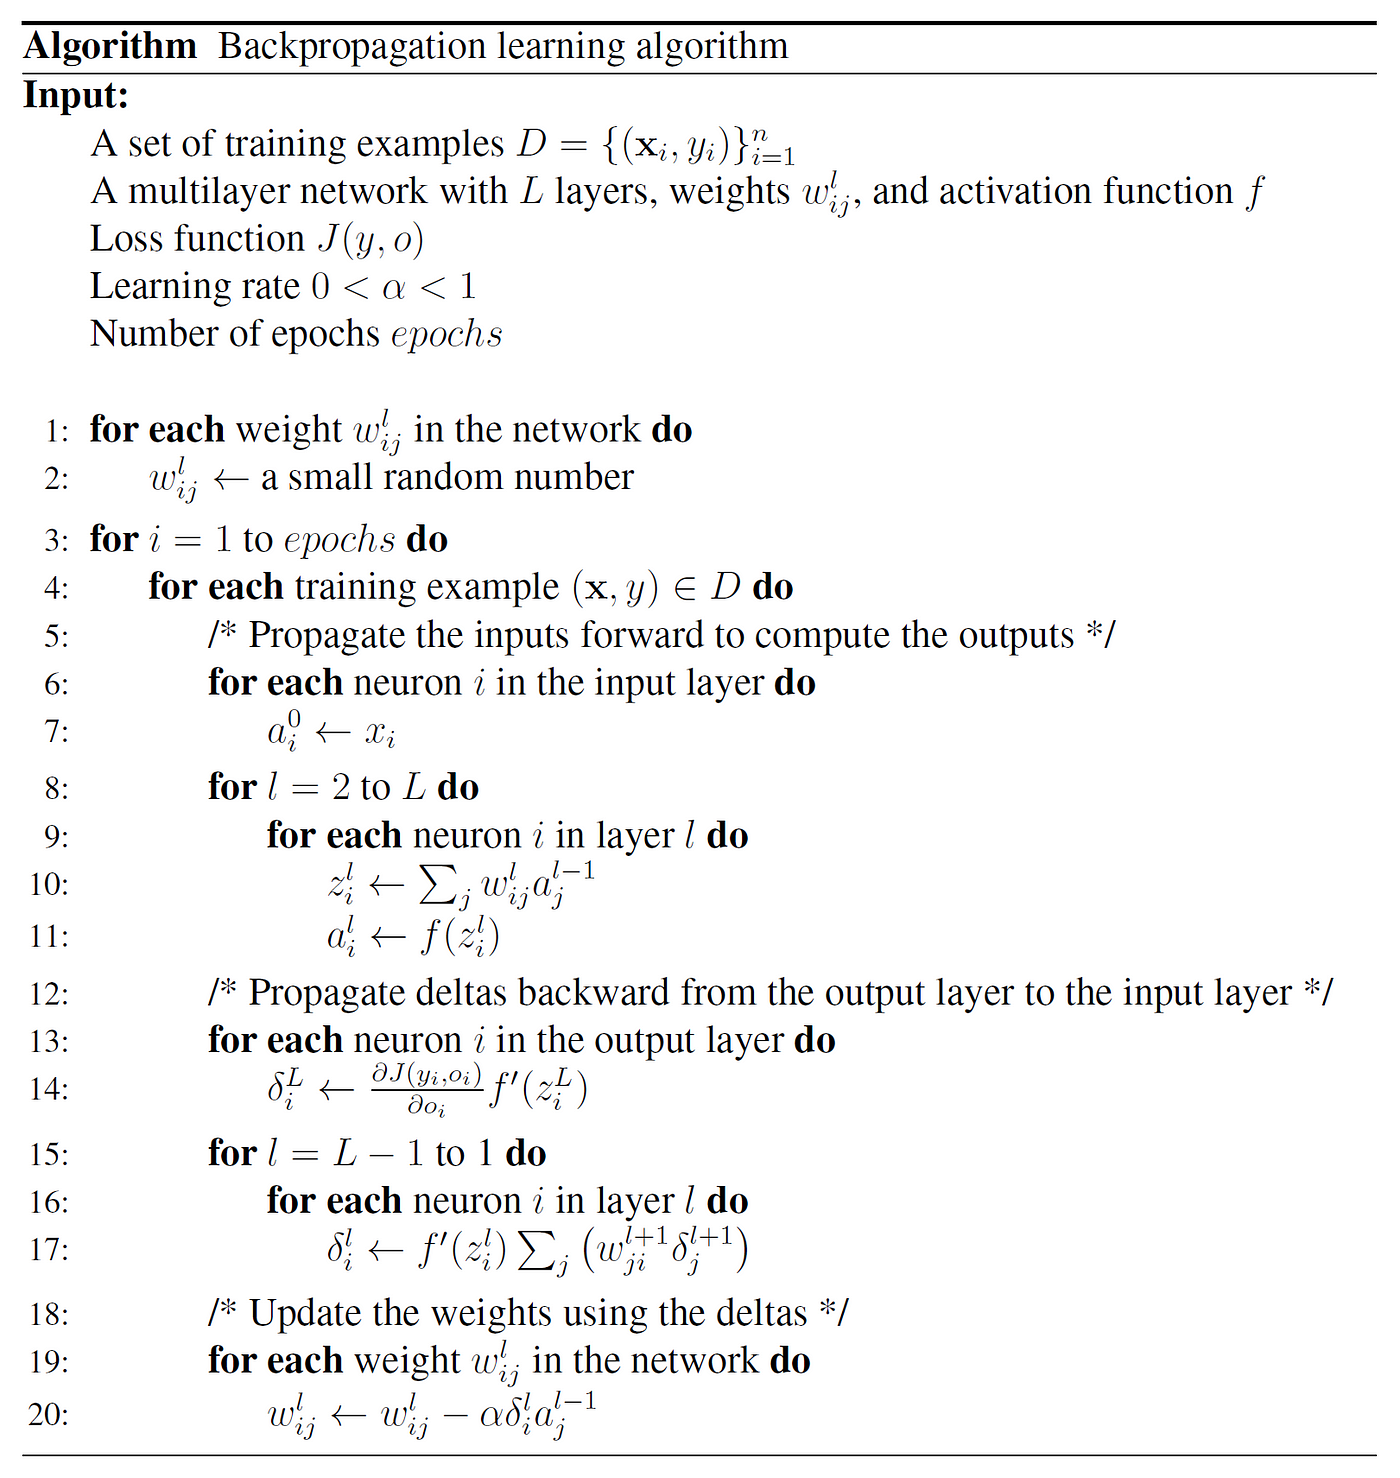
\includegraphics[scale=0.25]{/math/dl/backprop}
\caption{Backpropagation Algorithm}
\end{figure}

\begin{remark} \hlt{Backpropagation}\\
To calculate the gradient of loss function with respect to each of individual parameters of the neural network.\\
Model training begins with random initialisation of weights and biases.
\begin{enumerate}[label=\roman*.]
\setlength{\itemsep}{0pt}
\item Forward pass: input is sampled from training data. Nodes receive input vector and passes their value (multiplied by random initial weight) to nodes of first hidden layer. The hidden units take weighted sum of these output values as an input to the activation function, whose output is used for next hidden layer.
\item Error computation: the final output of the network is compared to the ground truth, difference is calculated for the error value.
\item Backwards pass: the error value computed earlier is used to compute the gradient of loss function. The gradient is then propagated back through the network, and the weights are updated according to their contribution to the error. The learning rate determines the size of weight updates.
\item Weights update: the weights are updated in opposite direction of the gradient
\end{enumerate}
\end{remark}


